% !TeX root = RJwrapper.tex
\title{ToOoOlTiPs: An R Package for Customizable Tooltips in Interactive
Graphics}
\author{by Quietest Quokka and Bounciest Bilby}

\maketitle

\abstract{%
An abstract of less than 150 words.
}

\hypertarget{introduction}{%
\section{Introduction}\label{introduction}}

Interactive data graphics provides plots that allow users to interact
them. One of the most basic types of interaction is through tooltips,
where users are provided additional information about elements in the
plot by moving the cursor over the plot.

This paper will first review some R packages on interactive graphics and
their tooltip implementations. A new package \CRANpkg{ToOoOlTiPs} that
provides customized tooltips for plot, is introduced. Some example plots
will then be given to showcase how these tooltips help users to better
read the graphics.

\hypertarget{background}{%
\section{Background}\label{background}}

Some packages on interactive graphics include \CRANpkg{plotly}
\citep{plotly} that interfaces with Javascript for web-based interactive
graphics, \CRANpkg{crosstalk} \citep{crosstalk} that specializes
cross-linking elements across individual graphics. The recent R Journal
paper \CRANpkg{tsibbletalk} \citep{RJ-2021-050} provides a good example
of including interactive graphics into an article for the journal. It
has both a set of linked plots, and also an animated gif example,
illustrating linking between time series plots and feature summaries.

\hypertarget{customizing-tooltip-design-with}{%
\section{\texorpdfstring{Customizing tooltip design with
\pkg{ToOoOlTiPs}}{Customizing tooltip design with }}\label{customizing-tooltip-design-with}}

\pkg{ToOoOlTiPs} is a packages for customizing tooltips in interactive
graphics, it features these possibilities.

\hypertarget{a-gallery-of-tooltips-examples}{%
\section{A gallery of tooltips
examples}\label{a-gallery-of-tooltips-examples}}

Figure \ref{fig:penguins-plotly} shows an interactive plot of the
\CRANpkg{palmerpenguins} data \citep{palmerpenguins}, made using the
\pkg{plotly} package.

\begin{Schunk}
\begin{Sinput}
p <- penguins %>% 
  ggplot(aes(x = bill_depth_mm, y = bill_length_mm, 
             color = species)) + 
  geom_point()
ggplotly(p)
\end{Sinput}
\begin{figure}
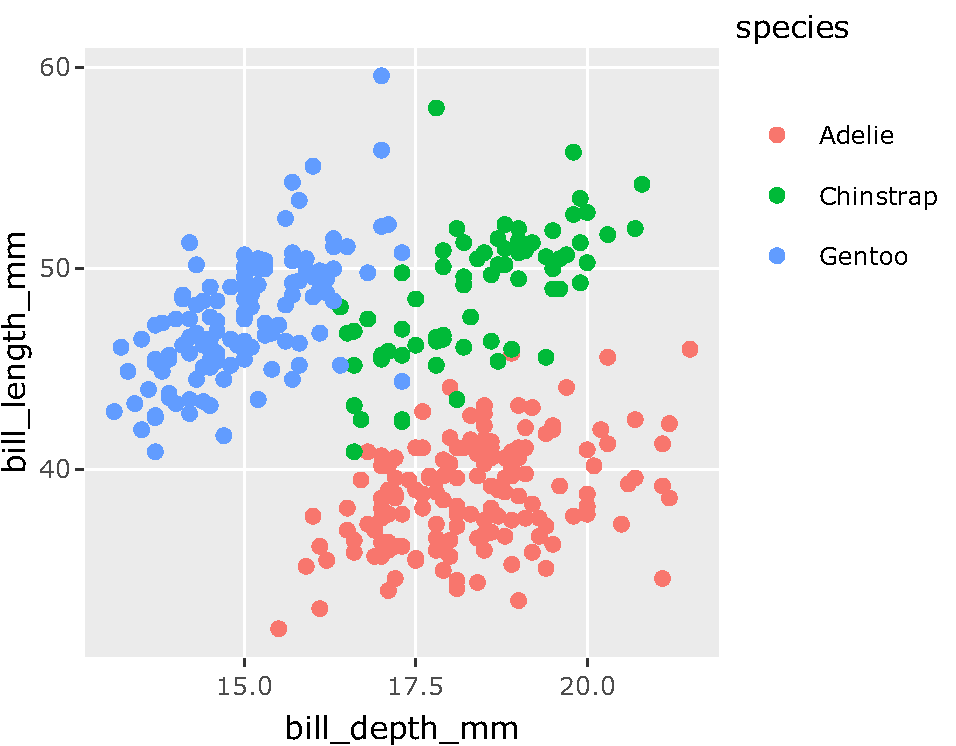
\includegraphics{sample-article_files/figure-latex/penguins-plotly-1} \caption[A basic interactive plot made with the plotly package on palmer penguin data]{A basic interactive plot made with the plotly package on palmer penguin data. Three species of penguins are plotted with bill depth on the x-axis and bill length on the y-axis. When hovering on a point, a tooltip will show the exact value of the bill depth and length for that point, along with the species name.}\label{fig:penguins-plotly}
\end{figure}
\end{Schunk}

\hypertarget{summary}{%
\section{Summary}\label{summary}}

We have displayed various tooltips that are available in the package
\pkg{ToOoOlTiPs}.

\bibliography{skeleton.bib}

\address{%
Quietest Quokka\\
University of Little Mates\\%
Department of Letter Q\\ Somewhere, Australia\\
%
\url{https://www.britannica.com/animal/quokka}\\%
\textit{ORCiD: \href{https://orcid.org/0000-1721-1511-1101}{0000-1721-1511-1101}}\\%
\href{mailto:qquo@ulm.edu}{\nolinkurl{qquo@ulm.edu}}%
}

\address{%
Bounciest Bilby\\
University of Little Mates\\%
Department of Letter B\\ Somewhere, Australia\\
%
\url{https://www.britannica.com/animal/bilby}\\%
\textit{ORCiD: \href{https://orcid.org/0000-0002-0912-0225}{0000-0002-0912-0225}}\\%
\href{mailto:bbil@ulm.edu}{\nolinkurl{bbil@ulm.edu}}%
}
